% !TeX encoding = UTF-8
% !TeX spellcheck = pl_PL

% $Id:$





\newcommand{\kurs}{Wizualizacja danych sensorycznych}
\newcommand{\formakursu}{Projekt}


\newcommand{\doctype}{Raport z rezultat\'{o}w projektu}




\newcommand{\projectname}{Wizualizacja warunk\'{o}w narciarskich w g\'{o}rach}






\newcommand{\osobaA}{Wojciech \textsc{Kosicki}, 234506}


\newcommand{\termin}{cz 18:55}


\newcommand{\prowadzacy}{Dr in\.{z}. Bogdan \textsc{Kreczmer}}

\documentclass[10pt, a4paper]{article}


%Preambuła dokumentu

% linki w spisie tresci, bibliografi
\usepackage[bookmarks=true,bookmarksnumbered=false,unicode=true,pdftex=true, colorlinks,filecolor=black,linkcolor=black,urlcolor=black,citecolor=black]{hyperref}

%ustawienie rozmiaru papieru
\usepackage[a4paper, left=2.5cm, right=2.5cm, top=2.5cm, bottom=2.5cm, headsep=1.2cm]{geometry}

%rozmaite ustawienia pozwalające okreslić język

%NALEŻY wybrać jeden z pakietów
%\usepackage{polski} %przydatne podczas składania dokumentów w j. polskim
\usepackage[polish]{babel}  % pakiet lokalizujący dokument w języku polskim
%\usepackage[british]{babel}

\usepackage{indentfirst}	% polski styl pisania (np. rozpoczecie pierwszego akapitu
% pod nazwa rozdzialu od wciecia)
%\usepackage[OT4]{fontenc}
\usepackage[utf8]{inputenc} % w miejsce utf8 można wpisać latin2 bądź cp1250,
% w zależności od tego w jaki sposób kodowane są 
% polskie znaki diakrytyczne przy wprowadzaniu 
% z klawiatury.
%kodowanie znaków, zależne od systemu
\usepackage[T1]{fontenc} %poprawne składanie polskich czcionek

%OPEROWANIE NA OBRAZACH
\usepackage{graphicx}       % pakiet graficzny, umożliwiający m.in.
% import grafik w formacie eps
%\usepackage{epstopdf}		% pozwala na importowanie grafik w formacie eps
% przy użyciu pdflatex
\usepackage[update,prepend]{epstopdf}
\usepackage{rotating}       % pakiet umożliwiający obracanie rysunków
\usepackage{subfigure}      % pakiet umożliwiający tworzenie podrysunków
\usepackage{epic}           % pakiet umożliwiający rysowanie w środowisku latex
\usepackage{psfrag}         % pakiet umożliwiający podmianę łańcuchów znaków 
% w plikach eps
%\usepackage{curves}         % pakiet do wykreslania krzywych

%pakiety dodające dużo dodatkowych poleceń matematycznych
\usepackage{amsfonts}       % pakiet z rozmaitymi czcionkami matematycznymi
%\usepackage{amssymb}        % pakiet z rozmaitymi symbolami matematycznymi
\usepackage{amsmath}        % pakiet z rozmaitymi środowiskami matematycznymi

\usepackage{fp}             % pakiet z funkcjami operujacymi 
% na liczbach zmiennoprzecinkowych
\usepackage{calc}           % pakiet umożliwiający operacje arytmetyczne
% na tzw. licznikach (liczbach całkowitych)
\usepackage{leftidx}		% indeksy górne i dolne po lewej stronie

%definicje matematyczne
\providecommand{\abs}[1]{\lvert#1\rvert}
\providecommand{\norm}[1]{\lVert#1\rVert}

%pakiety wspomagające i poprawiające składanie tabel
\usepackage{supertabular}
\usepackage{array}
\usepackage{tabularx}
\usepackage{hhline}
\usepackage{longtable}		% wsparcie dla dlugich tabel
\usepackage{multicol}		% podzial strony na wiele kolumn

%pakiet do BibTex
\usepackage{cite}

\usepackage{url} %pakiet pozawalający na dodawanie adresów url w bibliografi

%pakiet wypisujący na marginesie etykiety równań i rysunków zdefiniowanych przez \label{}, chcąc wygenerować finalną wersję dokumentu wystarczy usunąć poniższą linię
%\usepackage{showlabels}

\usepackage{float}			% lepsza obsluga mechanizmow obiektow plywajacych
% wymuszenie wstawienia np. tabeli, obrazka w danym miejscu przez [H]

\usepackage{listings}       % pakiet dedykowany zrodlom programow
\usepackage{color}


\definecolor{dkgreen}{rgb}{0,0.6,0}
\definecolor{gray}{rgb}{0.5,0.5,0.5}
\definecolor{mauve}{rgb}{0.58,0,0.82}

\lstset{ %
	language=Matlab,                % the language of the code
	basicstyle=\scriptsize,           % the size of the fonts that are used for the code
	numbers=left,                   % where to put the line-numbers
	numberstyle=\tiny\color{gray},  % the style that is used for the line-numbers
	stepnumber=1,                   % the step between two line-numbers. If it's 1, each line 
	% will be numbered
	numbersep=5pt,                  % how far the line-numbers are from the code
	backgroundcolor=\color{white},      % choose the background color. You must add \usepackage{color}
	showspaces=false,               % show spaces adding particular underscores
	showstringspaces=false,         % underline spaces within strings
	showtabs=false,                 % show tabs within strings adding particular underscores
	%frame=single,                   % adds a frame around the code
	rulecolor=\color{black},        % if not set, the frame-color may be changed on line-breaks within not-black text (e.g. comments (green here))
	tabsize=2,                      % sets default tabsize to 2 spaces
	captionpos=b,                   % sets the caption-position to bottom
	breaklines=true,                % sets automatic line breaking
	breakatwhitespace=false,        % sets if automatic breaks should only happen at whitespace
	%title=\lstname,                   % show the filename of files included with \lstinputlisting;
	% also try caption instead of title
	keywordstyle=\color{blue},          % keyword style
	commentstyle=\color{dkgreen},       % comment style
	stringstyle=\color{mauve},         % string literal style
	escapeinside={\%*}{*)},            % if you want to add LaTeX within your code
	morekeywords={*,...},              % if you want to add more keywords to the set
	deletekeywords={...}              % if you want to delete keywords from the given language
}

%polish signs in lst code
\lstset{literate=%
	{ą}{{\k{a}}}1
	{ć}{{\'c}}1
	{ę}{{\k{e}}}1
	{ł}{{\l}}1
	{ń}{{\'n}}1
	{ó}{{\'o}}1
	{ś}{{\'s}}1
	{ż}{{\.z}}1
	{ź}{{\'z}}1
	{Ą}{{\k{A}}}1
	{Ć}{{\'C}}1
	{Ę}{{\k{E}}}1
	{Ł}{{\L}}1
	{Ń}{{\'N}}1
	{Ó}{{\'O}}1
	{Ś}{{\'S}}1
	{Ż}{{\.Z}}1
	{Ź}{{\'Z}}1
}

\usepackage{verbatim}       % pakiet dedykowany rozmaitym wydrukom tekstowym
\usepackage{ifthen}         % pakiet umożliwiający tworzenie prostych programów
% (m.in. zawiera instrukcje powtórzeniowe 
% i warunkowe)
\usepackage{upquote}		%normal quotations marks ' and `

% deklaracje wymagane przez pakiet theorem automatycznie ladowany w przypadku
% klasy dokumentu article
%
\newtheorem{Dn}{Definicja}[section]     % deklaracja srodowiska definicja
\newtheorem{La}[Dn]{Lemat}                % deklaracja srodowiska lemat
\newtheorem{Tm}[Dn]{Twierdzenie}          % deklaracja srodowiska twierdzenie
\newtheorem{Rk}[Dn]{Spostrze{\.z}enie}  % deklaracja srodowiska spostrzezenie
\newtheorem{Am}[Dn]{Algorytm}           % deklaracja srodowiska algorytm
\newtheorem{As}[Dn]{Za{\l}o{\.z}enie}   % deklaracja srodowiska zalozenie
\newtheorem{Pn}[Dn]{Propozycja}           % deklaracja srodowiska propozycja
\newtheorem{Py}[Dn]{W{\l}asno{\'s}{\'c}}  % deklaracja srodowiska wlasnosc
\newtheorem{Cy}[Dn]{Wniosek}              % deklaracja srodowiska wniosek
\newtheorem{Ee}[Dn]{Przyk{\l}ad}        % deklaracja srodowiska przyklad
\newtheorem{Ex}{{\'C}wiczenie}          % deklaracja srodowiska cwiczenie

%helps to specify width of a column in table
%\begin{tabular}{|C{1cm}|c|c|c|c|c|c|c|c|c|c|}
%first column will have widht of 1cm
\newcolumntype{L}[1]{>{\raggedright\let\newline\\\arraybackslash\hspace{0pt}}m{#1}}
\newcolumntype{C}[1]{>{\centering\let\newline\\\arraybackslash\hspace{0pt}}m{#1}}
\newcolumntype{R}[1]{>{\raggedleft\let\newline\\\arraybackslash\hspace{0pt}}m{#1}}

\sloppy			%zawija bardzo długie linie

%\pagenumbering{gobble}% Remove page numbers (and reset to 1)

	
\begin{document}

\def\tablename{Tabela}	

\begin{titlepage}
	\begin{center}
		\textsc{\LARGE \formakursu}\\[1cm]		
		\textsc{\Large \kurs}\\[0.5cm]		
		\rule{\textwidth}{0.08cm}\\[0.4cm]
		{\huge \bfseries \doctype}\\[1cm]
		{\huge \bfseries \projectname}\\[0.5cm]
	
		\rule{\textwidth}{0.08cm}\\[1cm]
		
		\begin{flushright} \large
		\emph{Skład grupy:}\\
		\osobaA\\

		
		\emph{Termin: }\termin\\[0.4cm]

		\emph{Prowadzący:} \\
		\prowadzacy \\
		
		\end{flushright}
		
		\vfill
		
		{\large \today}
	\end{center}	
\end{titlepage}

\newpage
\tableofcontents
\newpage

\section{Wstęp}
\label{sec:OpisProjektu}
Dokument został stworzony jako sprawozdanie z prawie końcowego etapu realizacji projektu pt. "Wizualizacja warunków narciarskich w górach". Projekt jest realizowany w qt Creator 4.5.1. Raport ten omawia przebieg prac oraz określa co udało się zrealizować z założeń projektu. Jest to też ostateczny raport końcowy.

\section{Implementacja okien aplikacji} 
Zakończono prace nad wyglądem okna Domyślnego i okna Szczytu aplikacji. Usunięto obszary testowe i ułożono wszystkie elementy typu Widget. Program w celach prezentacyjnych zawiera cztery szczyty, Karpacz, Szczyrk, Krynicę oraz Zieleniec. Na głównym oknie wyświetlane są dane o zachmurzeniu, temperaturze, stanie zaśnieżenia stoku oraz ogólny stan pogodowy na szczycie. Aby wyświetlić dokładniejsze informacje o warunkach panujących na danym wzgórzu, trzeba kliknąć jego symbol na mapie. Można otworzyć kilka szczytów naraz w różnych oknach. Wybierając pozycję w Menu o nazwie Aktualizacja danych, dokonuje się pobrania danych z portalu internetowego dostarczających informacji pogodowych. Wybierając z kolei opcję w Menu, Zmiana widoku mapy, można zmienić wygląd mapy Polski z graficznej na geograficzną i z powrotem. Zarówno okno Szczytu jak i okno Domyślne mają na stałe ustawione wymiary 1200x500 pikseli. 


\section{Pobranie danych ze strony internetowej} 
Program wykorzystuje biblioteki QNetworkAccessManager, QNetworkRequest oraz QNetworkReply by pobrać kod źródłowy strony o podanym url. 
Aplikacja ściąga kod źródłowy strony internetowej z odpowiednimi danymi o warunkach pogodowych na danym szczycie. Kod, po odpowiednim wyselekcjonowaniu istotnego fragmentu jest zapisywany w pliku .txt. Do wyboru odpowiedniego fragmentu kodu wykorzystano bibliotekę QRegExp, służącą do parsowania danych ze zmiennej QString. 

\section{Parsowanie danych} 
Po ściągnięciu odpowiedniego fragmentu kodu źródłowego należało wyciągnąć odpowiednie zmienne z jego zawartości. Do parsowania danych wykorzystaną tę samą bibliotekę, która została wykorzystana do zapisania w pliku .txt odpowiedniego fragmentu kodu, QRegExp. QRegExp daje szerokie możliwości do wyszukiwania odpowiednich określeń w tekście, parsowania danych lub modyfikacji danych typu QString. 
\section{Ocena jakości szczytu} 
Program ma za zadanie oceniać ogólną jakość warunków narciarskich na danym szczycie.
Każdej danej uzyskanej z kodu źródłowego przypisano wartość punktową. Rozdzielenie wartości punktowych jest uzależnione od specyfikacji danej. W punktacji uwzględniona została waga danego warunku atmosferycznego (np. temperatura jest o wiele bardziej istotna niż ciśnienie) oraz wyjątki (np. opady są pozytywnie punktowane tylko przy ujemnej temperaturze).
W celu określenia jakości pogodowych na danym szczycie, napisano funkcję algorytm(). Ma ona za zadanie przyjąć punktowe wartości danych warunków atmosferycznych i określić stan szczytu. 
\section{Prace graficzne} 
Grafiki testowe, które zostały wykonane w programie Paint, zostały zastąpione grafikami zrealizowanymi w Inkspace. Poszczególne obrazy typu .PNG stworzono od podstaw wykorzystując możliwości oprogramowania graficznego Inkspace oraz w mniejszym stopniu Gimp.Nie stworzono jednak ich w formie przeźroczystego tła, aby zachowały swoją czytelność, nawet przy zmianie widoku mapy na graficzny.  

\newpage
\section{Obecny roboczy wygląd aplikacji} 
	\begin{figure}[!h]
	\centering
	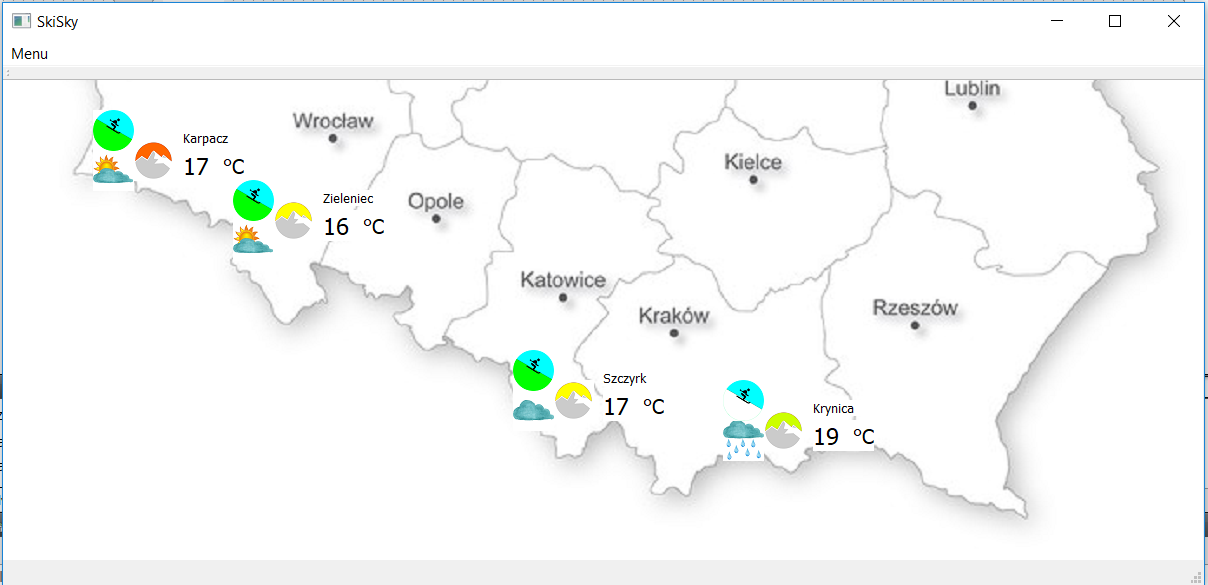
\includegraphics[width=\linewidth]{02.png}
	\caption{Główne okno z mapą graficzną}
	\end{figure}
	
	\begin{figure}[!h]
	\centering
	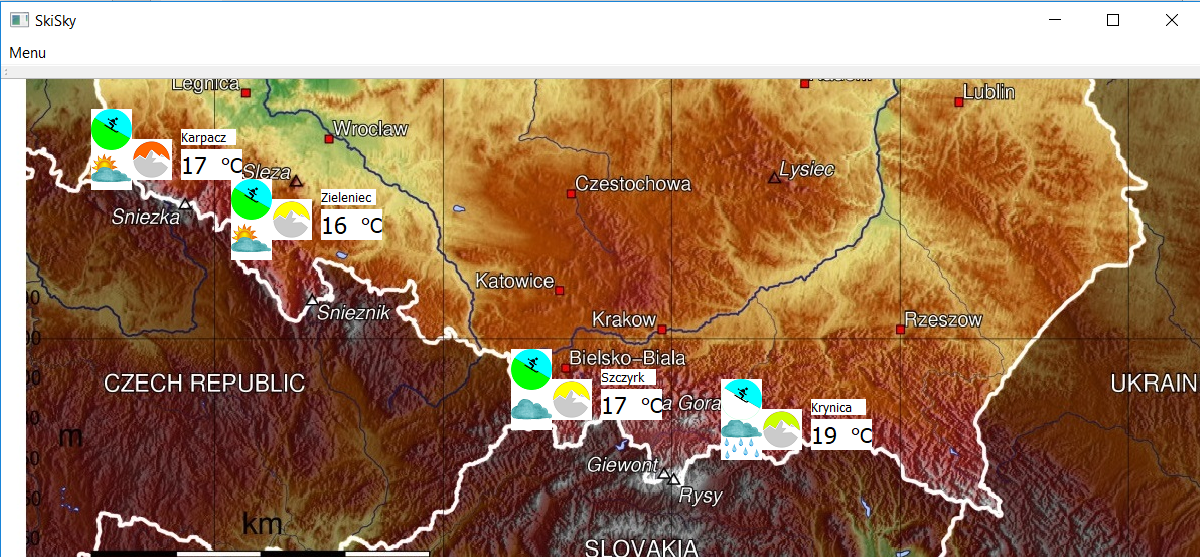
\includegraphics[width=\linewidth]{03.png}
	\caption{Główne okno z mapą geograficzną}
	\end{figure}
	\begin{figure}[!h]
	\centering
	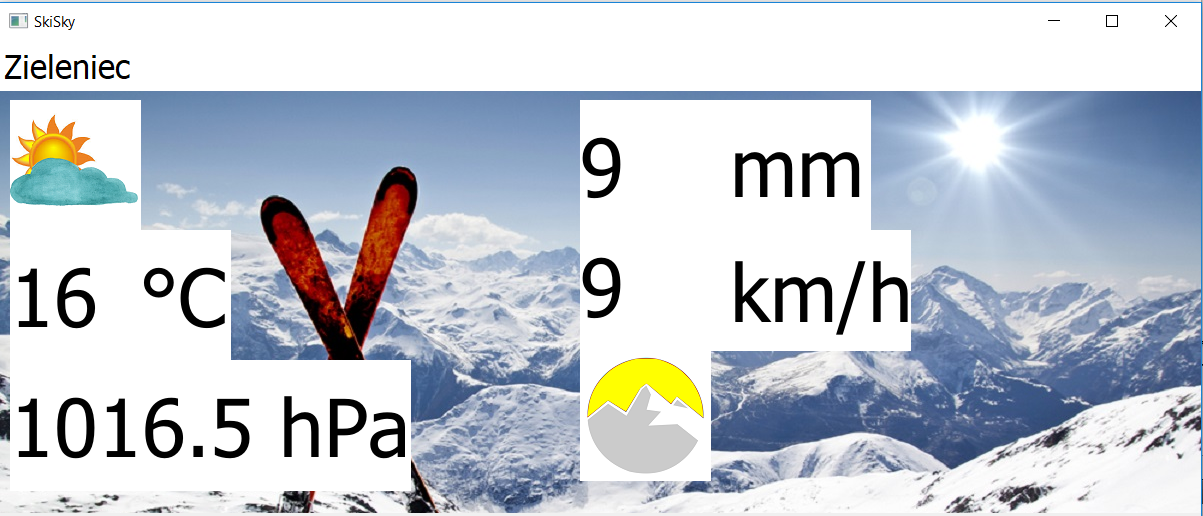
\includegraphics[width=\linewidth]{04.png}
	\caption{Okno szczytu Zieleniec}
	\end{figure}
\newpage
\newpage
\newpage
\section{Podsumowanie} 
Projekt pt. Wizualizacja warunków narciarskich w górach został zrealizowany w większości założeń projektowych. Udało się zaimplementować pobieranie i parsowanie danych od serwisu zewnętrznego. Za pomocą bibliotek Qt stworzono aplikację, która w przejrzysty sposób przedstawia pogodę na wybranym szczycie i daje szybka przejrzystą ocenę szczytu. Założenia projektowe trzeba było lekko zweryfikować i zmodyfikować w fazie realizacji projektu. Pd koniec marca zaobserwowano zamknięcie serwisu pogodowego z którego miały być pobierane początkowo dane. Dlatego trzeba było wybrać inny serwis internetowy i dobrać innego typu dane. Zabrakło teraz min. liczby aktywnych wyciągów. Aplikację testowano na niewielkiej próbce użytkowników w liczbie 33. W skład ich wchodziło 11 studentów (wiek 19-21 lat), 11 licealistów (wiek 16-18 lat) oraz 11 osób pracujących (wiek 24-34 lat). Wszyscy badani potwierdzili, że regularnie wyjeżdżają w góry na narty. Poniżej zamieszczono wyniki ankiety. Jak widzimy, aplikacja najlepiej została oceniona przez ludzi pracujących. Aczkolwiek uzyskana różnica w ocen między studentami i pracującymi, może być przypadkowa przy tak małej próbce. Mimo to można stwierdzić, że aplikacja spotkała się z pozytywną oceną. Rzadko zdarzały się wyniki poniżej 3 punktów na 5. To na co zwracali przede wszystkim użytkownicy to brak możliwości sprawdzenia aktywnych wyciągów oraz brak możliwości sprawdzenia większej liczby szczytów. Liczba szczytów ograniczona do czterech była przyjęta w założeniach projektowych. Założono, że nie ma potrzeby implementować więcej szczytów na wersje prototypową aplikacji. Z kolei brak informacji o aktywnych wyciągach jest wynikiem ograniczonych możliwości serwisu zewnętrznego. Ku zaskoczeniu, żaden użytkownik nie skrytykował graficznego wyglądu aplikacji, mimo nie zaimplementowania przeźroczystego tła dla grafik oraz braku animacji. Trudności ze zrealizowaniem tych dwóch elementów wynikały ze złego zaplanowania terminów realizacji projektu oraz wzrostu obciążenia zasobu czasu w okresie od 1 czerwca do 21 czerwca. 
	\begin{figure}[!h]
	\centering
	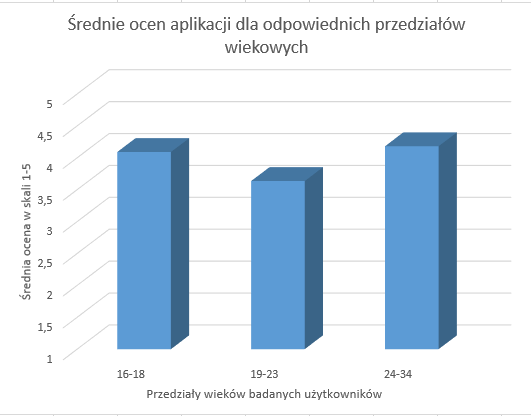
\includegraphics[width=\linewidth]{w1.png}
	
	\end{figure}
		\begin{figure}[!h]
	\centering
	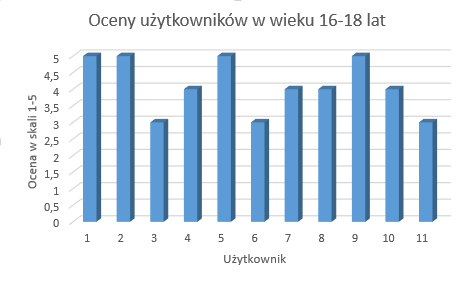
\includegraphics[width=\linewidth]{w2.png}

	\end{figure}
	\begin{figure}[!h]
	\centering
	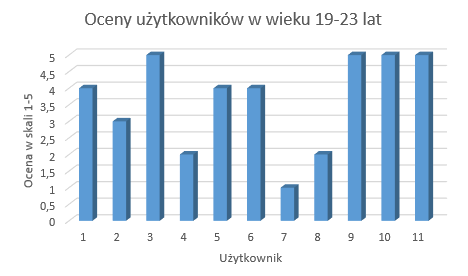
\includegraphics[width=\linewidth]{w3.png}
	
	\end{figure}
	\begin{figure}[!h]
	\centering
	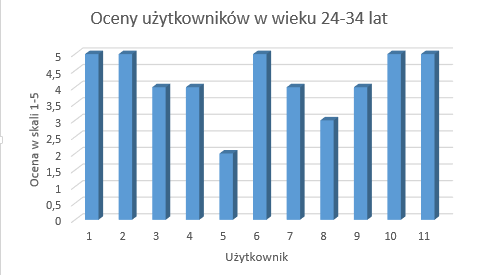
\includegraphics[width=\linewidth]{w4.png}

	\end{figure}

\addcontentsline{toc}{section}{Bibilografia}
\bibliography{bibliografia}
\bibliographystyle{plain}


\end{document}







































